\fuxiti
\begin{xiaotis}

\xiaoti{下列的说法哪一种是正确的?为什么?}
\begin{xiaoxiaotis}

    \xxt{空气是一种元素,}
    \xxt{空气是一种化合物,}
    \xxt{空气是几种元素的混和物,}

    \xxt{空气是几种化合物的混和物,}
    \xxt{空气是几种单质和几种化合物的混和物。}

\end{xiaoxiaotis}


\xiaoti{有三个集气瓶,分别充满空气、氮气和氧气。试用简单的方法加以鉴别。}


\xiaoti{燃着的蜡烛放入氮气或氩气里就会熄灭,为什么电灯泡里还要填充氮气和氩气?}


\xiaoti{下列的物质里哪些存在着氧气分子,为什么?}
\begin{xiaoxiaotis}

    \xxt{二氧化锰(\ce{MnO2}),}
    \xxt{空气,}
    \xxt{贮存在钢瓶里的氧。}

\end{xiaoxiaotis}


\xiaoti{有人画了下面的关于实验室里制取氧气的装置图,回答以下两个问题:}
\begin{xiaoxiaotis}

    \xxt{这个图是否有错误?如果有错误,指出错误在哪里,并说明改正的方法。}

    \begin{figure}[H]
        \centering
        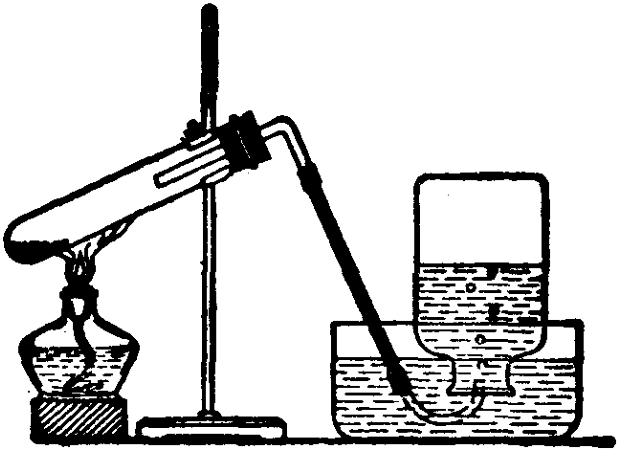
\includegraphics[width=9cm]{../pic/czhx1-ch1-fuxi-5}
    \end{figure}


    \xxt{实验完毕后,应该先移去酒精灯还是先把导管从水里拿出来?为们么?}

\end{xiaoxiaotis}


\xiaoti{根据二氧化碳的分子式,计算:}
\begin{xiaoxiaotis}

    \xxt{二氧化碳里碳元素和氧元素的质量比。}

    \xxt{二氧化碳里各元素的百分含量。}

    \xxt{$11$ 克二氧化碳里含碳多少克。}

    \xxt{多少克二氧化碳里含有 $6$ 克碳。}

\end{xiaoxiaotis}


\xiaoti{用在空气里燃烧锌的方法生产氧化锌(\ce{ZnO}),制得的氧化锌的质量比金属锌增大了。
    试解释这种现象。写出这个反应的化学方程式,并指出反应物、生成物各物质之间的质量比。
}


\xiaoti{配平化学方程式时,为什么不能改动分子式里表示原子个数的小数字?}


\xiaoti{为什么用下列几个化学方程式来表示氯酸钾受热分解放出氧气的反应都是错误的?
    \begin{fangchengshi}
        \ce{KClO3
            $\xlongequal[\Delta]{\ce{MnO2}}$
            KCl + 3O
        } \\
        \ce{KClO3
            $\xlongequal[\Delta]{\ce{MnO2}}$
            KCl + O2
        } \\
        \ce{KClO3
            $\xlongequal[\Delta]{\ce{MnO2}}$
            KClO + O2
        } \\
        \ce{KClO3
            $\xlongequal[\Delta]{\ce{MnO2}}$
            KCl + O2
        }
    \end{fangchengshi}
    写出实验室里给氯酸钾加热制取氧气的反应的化学方程式。
}


\xiaoti{计算氧化铁(\ce{Fe2O3}) 里铁元素和氧元素的百分含量。
    如果需要生产 $20$ 吨铁,那么至少需要多少吨氧化铁?
}

\end{xiaotis}

